\section{Experimental Evalutation}

\subsection{Communication cost of the consensus protocol}

\begin{figure}[tb]
  \centering
  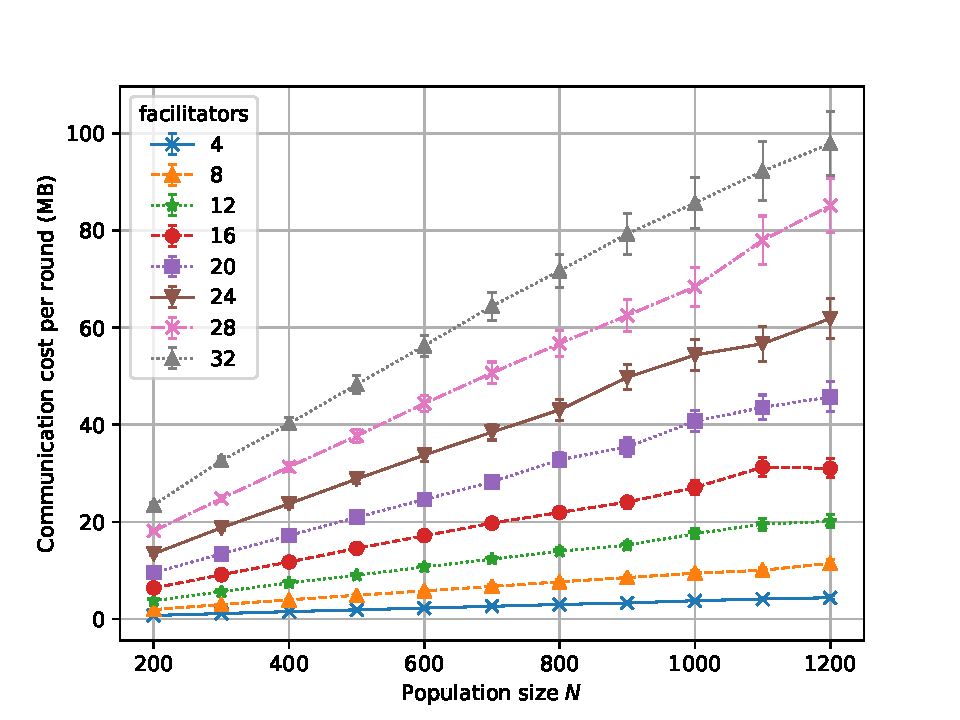
\includegraphics[width=\linewidth]{neighbour-random/round-communication-cost-vs-population}
  \caption{Communication cost for the consensus protocol per round increases linearly with population size.
  The error bars are larger for higher population size or higher number of facilitators is because rounds take longer thus they are repeated fewer times.}
  \label{fig:round-comms}
\end{figure}

\begin{figure}[tb]
  \centering
  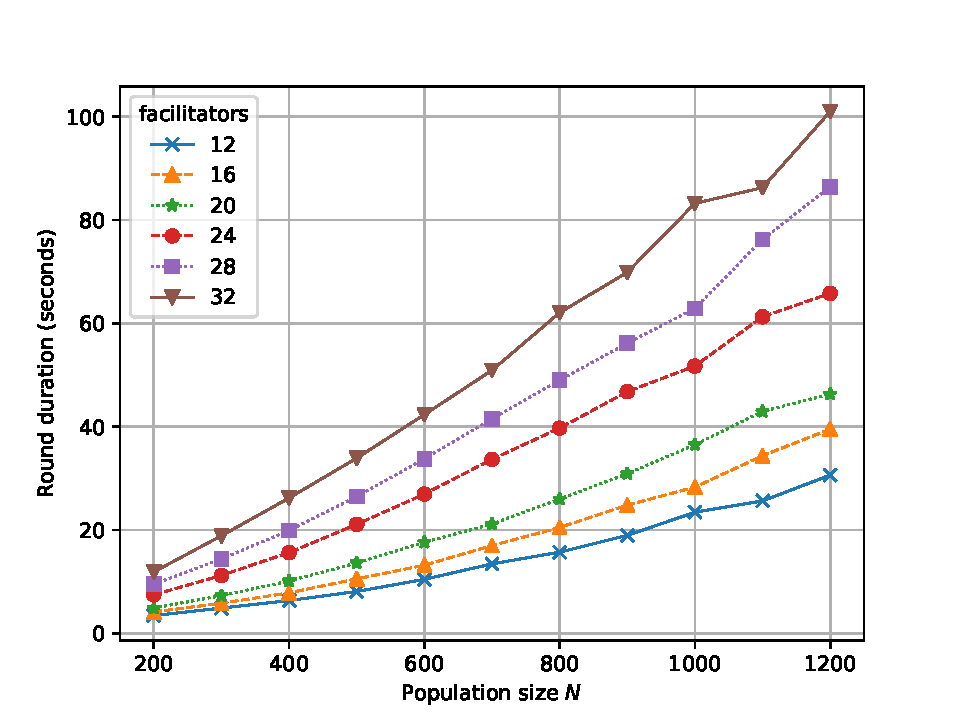
\includegraphics[width=\linewidth]{neighbour-random/round-duration-vs-population}
  \caption{Round duration does not increase linearly with the population size. 
  This is likely due to the additional hashing operation required for larger consensus result.}
  \label{fig:round-duration}
\end{figure}

\Cref{fig:round-comms} shows the relationship between the communication cost of the consensus protocol per round and the population size.
The most important aspect is that these results show a linear increase.
This reinforces our analytical result in~\Cref{sec:cons-complexity}.
Note that regardless of whether the transactions are performed with a random neighbour or with a fixed neighbour,
the magnitude of the communication cost is similar.
Both peak at about 100 MB.
This is expected because the consensus protocol is decoupled from the transaction protocol and the validation protocol.
Finally, the rate for which the communication cost increases is higher when the number of facilitators is higher.
This is also expected because the ACS algorithm has an $n^2$ term in its communication complexity.

We are also interested in how communication costs translate to time.
Hence, for the same experiment, we record the duration in seconds and the result is shown in~\Cref{fig:round-duration}.
Interestingly, the duration is not entirely linear.
We attribute this behaviour to the extra time needed to hash the CP blocks in the consensus result to compute the luck value.
Since if $N$ increases, every node must also perform more hash operations.
These results do not conform to analytical result in~\Cref{sec:cons-duration}.
Nevertheless, the difference is minor and there are ways to optimise the luck value computation.
For example, the luck value can be computed by the facilitators and are sent with the consensus result.
Then the non-facilitator nodes simply use it if there are enough signatures.

\subsection{Communication cost of transaction and validation}
\begin{figure}[h]
  \centering
  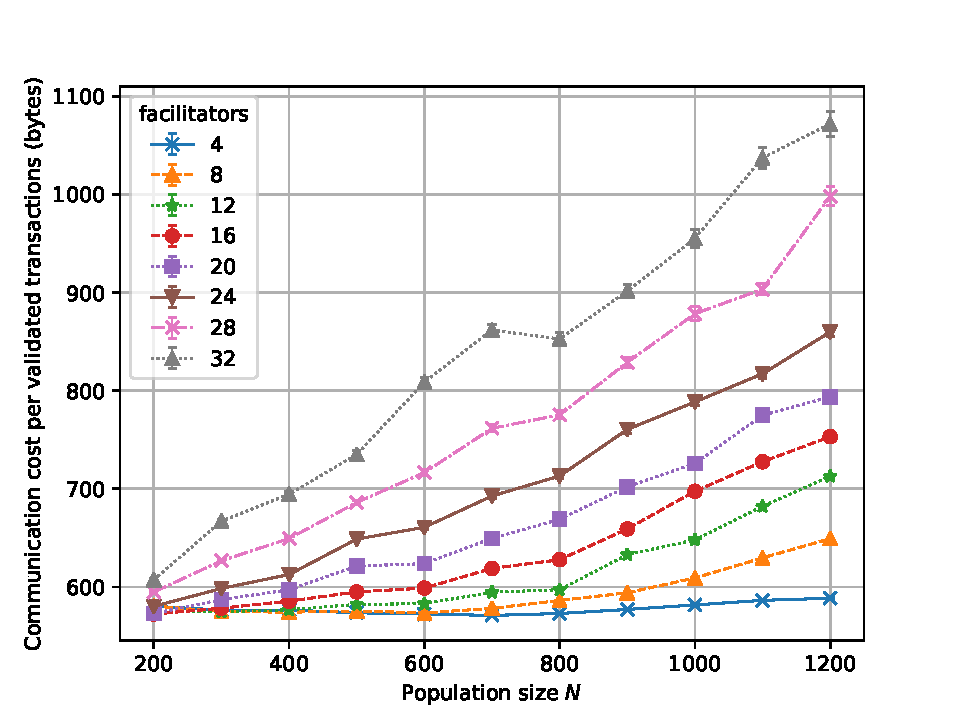
\includegraphics[width=\linewidth]{neighbour-random/tx-communication-cost-vs-population}
  \caption{Communication cost per verified transaction has similar (near linear) trend as~\Cref{fig:round-duration}.
  Fluctuation for the fixed-neighbour mode exists because the cache mechanism is unpredictable.}
  \label{fig:tx-comms}
\end{figure}

\subsection{Linear Global Throughput}

\begin{figure}[h]
  \centering
  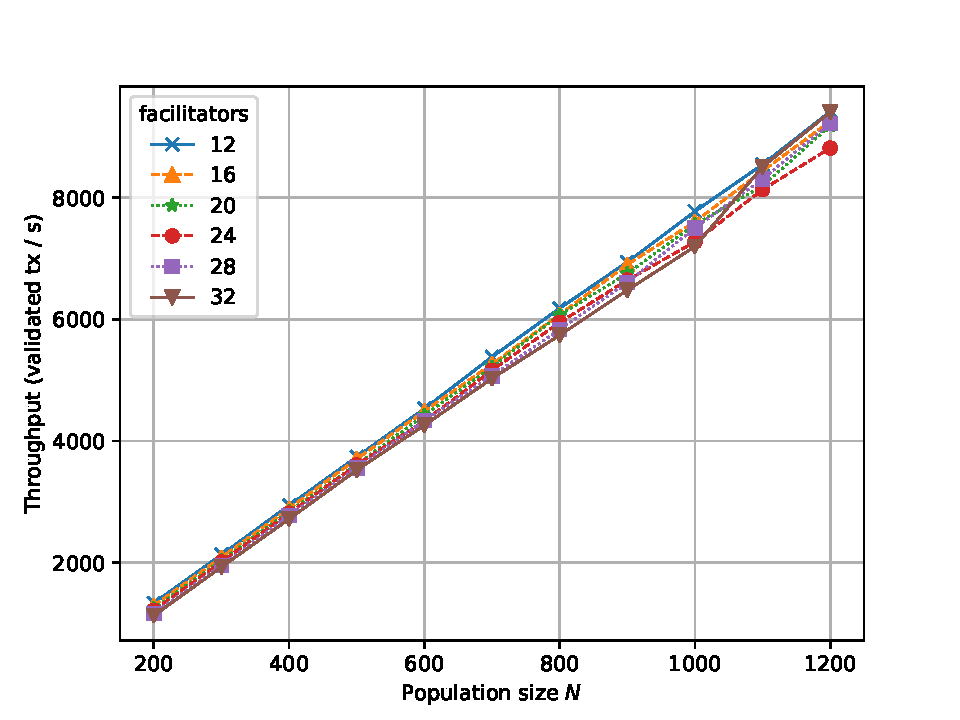
\includegraphics[width=\linewidth]{neighbour-random/throughput-vs-population}
  \caption{Global throughput increases as the population increases when every node transact at the same rate.
  Using fixed neighbours results in a higher throughput because of the caching mechanism.}
  \label{fig:global-throughput}
\end{figure}


Finally, the global throughput results are shown in~\Cref{fig:global-throughput}.
Evidently, the throughput has a linear relationship with the population size.
This result is a strong indication of the horizontal scalability which we aimed to achieve.
